\section{Computational illustration}

To illustrate the behaviour of the split bound, we consider a simple
Gaussian process design problem on a finite candidate set.

We sample $M=3000$ candidate locations uniformly from $[0,1]^2$
and select a budget of $N=100$ observations.
The underlying Gaussian process uses a squared exponential kernel with
lengthscale $\ell=0.12$, unit signal variance and observation noise
variance $\sigma^2=0.02$.

In both experiments below we compare a smooth Gaussian weight function
with a piecewise constant two-region overestimate. The latter is chosen
so that
\begin{equation*}
w_{\mathrm{clip}}(x)\geq w_{\mathrm{gauss}}(x)
\end{equation*}
for every candidate location, allowing the split bound developed in the
previous sections to be applied.

Since exact computation of maximum information gain is combinatorial in
the number of candidate points, all information-gain quantities reported
here are greedy approximations. The purpose of the experiment is not to
estimate the exact values of the bounds, but rather to investigate how
the split bound behaves relative to the corresponding crude bound.
\subsection{Localised high-weight region}

We first consider a Gaussian weight centred at a single point,
\begin{equation*}
w_{\mathrm{gauss}}(x)
=
a\exp\!\left(
-\frac{\|x-c\|^2}{2s^2}
\right),
\end{equation*}
with
\begin{equation*}
a=2,
\qquad
c=(0.78,0.72),
\qquad
s=0.10.
\end{equation*}

As before, we construct a two-region overestimate
\begin{equation*}
w_{\mathrm{clip}}(x)
=
\begin{cases}
a,& \|x-c\|\le r,\\
b,& \text{otherwise},
\end{cases}
\end{equation*}
with $b=0.5$ and
\begin{equation*}
r=s\sqrt{2\log(a/b)}.
\end{equation*}

This partitions the domain into a high-weight region $A$ and a background region $B$, containing $256$ and $2744$ candidate points respectively.

\begin{figure}[H]
\centering
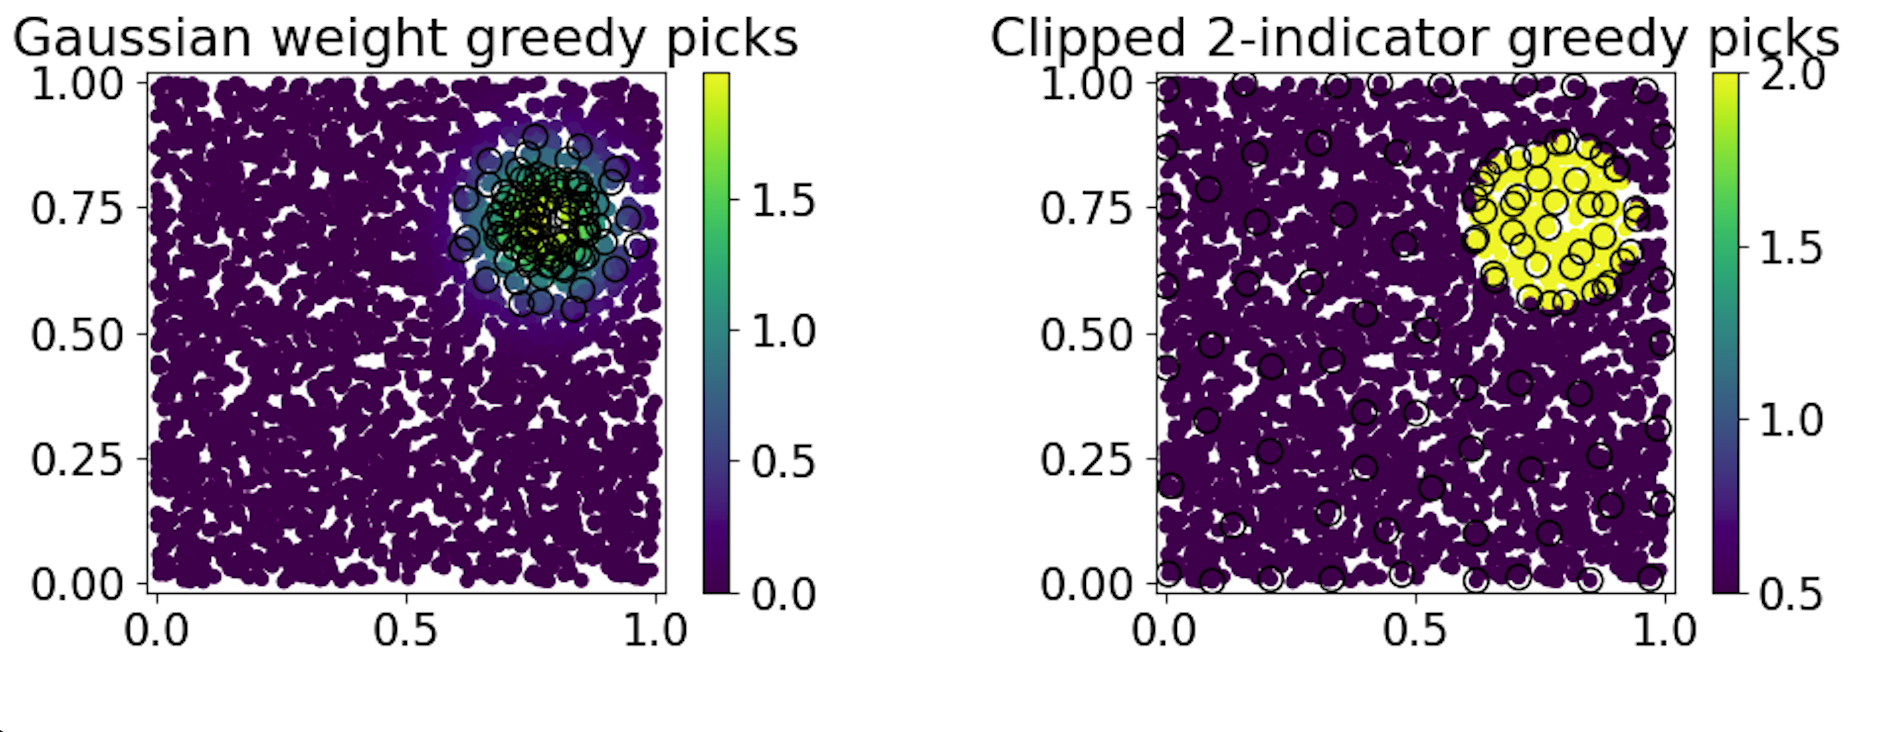
\includegraphics[width=0.9\linewidth]{point1.png}
\caption{
Gaussian weight centred at a point and the corresponding clipped two-region overestimate. Circles indicate the locations selected by the greedy weighted design.
}
\label{fig:point_geometry}
\end{figure}

Figure~\ref{fig:point_geometry} shows that both weighting schemes concentrate the selected points near the region of interest. Under the Gaussian weight, $93$ of the $100$ selected points lie inside the high-weight region.

The resulting greedy weighted objectives were
\begin{equation*}
\Gamma_{\mathrm{gauss}}^{\mathrm{greedy}}
=
65.89,
\qquad
\Gamma_{\mathrm{clip}}^{\mathrm{greedy}}
=
204.85.
\end{equation*}

The optimal split occurred at $m=22$, yielding
\begin{equation*}
\widehat B_{\mathrm{split}}
=
213.03,
\end{equation*}
compared with the crude bound
\begin{equation*}
\widehat B_{\mathrm{crude}}
=
385.29.
\end{equation*}

Thus the split bound reduces the crude bound by approximately $45\%$.

\begin{figure}[H]
\centering
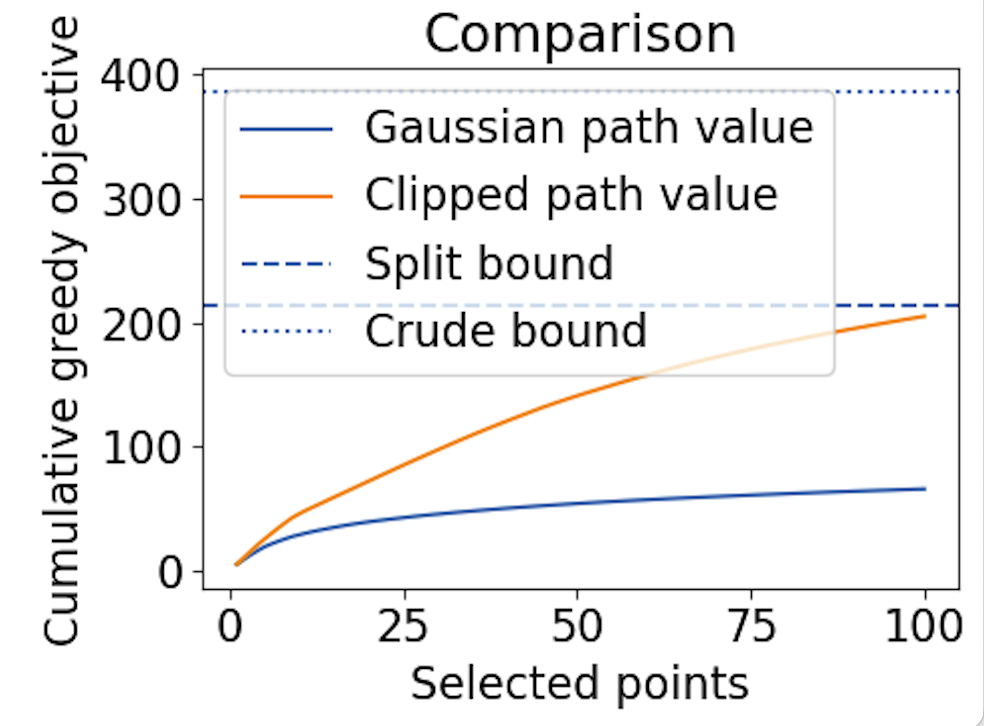
\includegraphics[width=0.5\linewidth]{point2.png}
\caption{
Cumulative greedy objective values together with the split and crude bounds.
}
\label{fig:point_bounds}
\end{figure}

Figure~\ref{fig:point_bounds} shows that the split bound tracks the clipped-weight objective much more closely than the crude max-weight bound. The improvement arises because the high-weight region occupies only a small fraction of the domain, allowing the regional decomposition to exploit this localisation.

\subsection{High-weight tube around a one-dimensional structure}

Our second experiment considers a weight concentrated around the line
\begin{equation*}
L=\{(x,y)\in[0,1]^2:y=0.5\}.
\end{equation*}

The Gaussian weight is defined by
\begin{equation*}
w_{\mathrm{gauss}}(x,y)
=
a
\exp\!\left(
-\frac{d_L(x,y)^2}{2s^2}
\right),
\end{equation*}
where
\begin{equation*}
d_L(x,y)=|y-0.5|.
\end{equation*}

The corresponding clipped overestimate is obtained using the same parameters as in the previous experiment. This produces a high-weight band containing $774$ candidate points and a background region containing $2226$ candidate points.

\begin{figure}[H]
\centering
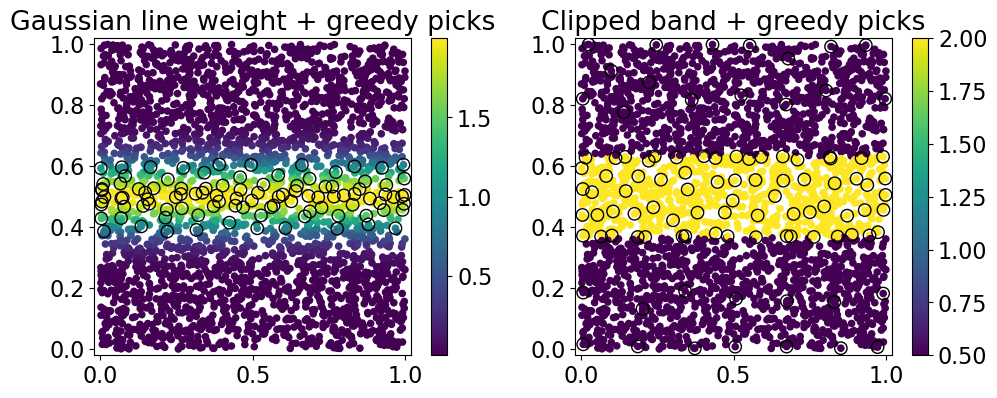
\includegraphics[width=0.9\linewidth]{line1.png}
\caption{
Gaussian line weight and clipped band approximation together with the greedy sampling locations.
}
\label{fig:line_geometry}
\end{figure}

As shown in Figure~\ref{fig:line_geometry}, the greedy weighted design strongly concentrates its samples inside the band. Under the Gaussian weight all $100$ selected points lie inside the high-weight region.

The greedy weighted objectives were
\begin{equation*}
\Gamma_{\mathrm{gauss}}^{\mathrm{greedy}}
=
165.60,
\qquad
\Gamma_{\mathrm{clip}}^{\mathrm{greedy}}
=
264.61.
\end{equation*}

The best split occurred at $m=42$, yielding
\begin{equation*}
\widehat B_{\mathrm{split}}
=
271.16,
\end{equation*}
while the crude bound remained
\begin{equation*}
\widehat B_{\mathrm{crude}}
=
385.29.
\end{equation*}

This corresponds to a reduction of approximately $30\%$.

\begin{figure}[H]
\centering
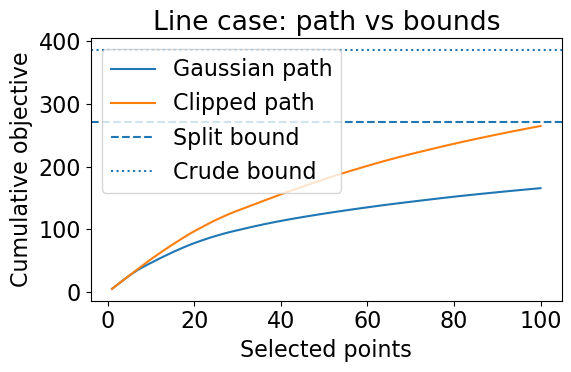
\includegraphics[width=0.5\linewidth]{line2.png}
\caption{
Cumulative greedy objective values together with the split and crude bounds.
}
\label{fig:line_bounds}
\end{figure}

\subsection{Discussion}

Both experiments exhibit a substantial gap between the split and crude
bounds. The effect is strongest in the first experiment, where the
high-weight region occupies a small localised subset of the domain and
the split bound improves the crude bound by approximately $45\%$.

In the second experiment the high-weight region occupies a much larger
fraction of the domain, leading to a smaller but still significant
improvement of approximately $30\%$.

These observations are consistent with the theoretical results of the
previous sections. When the regions carrying the largest weights occupy
only a small portion of the domain, analysing them separately can yield
considerably tighter information-gain estimates than treating the entire
domain as though it were weighted uniformly by the largest weight.
